\documentclass{beamer}
\usepackage[normalem]{ulem}
\usepackage[absolute,overlay]{textpos}
%\usetheme{Singapore}

\usepackage{pgfplots}
\pgfplotsset{compat=1.18}

%\include{preamble}

\usepackage{svg}

   
%\usecolortheme[RGB={204,51,255}]{structure}
%\usecolortheme[named=purple]{structure}
\usecolortheme[RGB={62,128,62}]{structure}
%\definecolor{dark}{rgb}{0.3,0.15,0.3}
%\definecolor{light}{rgb}{0.8,0.6,0.8}
\definecolor{reddish}{rgb}{.5,0.15,0.15}
\definecolor{rr}{rgb}{.5,0.15,0.15}
\definecolor{dark}{rgb}{0.4,0.2,0.4}
\definecolor{darkgreen}{rgb}{0.25,0.5,0.25}
\definecolor{darkred}{rgb}{0.75,0.25,0.25}
\definecolor{darkblue}{rgb}{0.25,0.25,0.75}
\definecolor{light}{rgb}{0.8,0.6,0.8}
\definecolor{reddish}{rgb}{.7,0.25,0.25}


\newcommand{\cored}{\color{red}{}}
\newcommand{\coblu}{\color{blue}{}}
\newcommand{\coblue}{\color{blue}{}}
\newcommand{\cor}{\color{reddish}{}}
\newcommand{\cob}{\color{black}{}}

\newcommand{\mm}[1]{\color{reddish}{}$#1$\color{black}{}}

\renewcommand{\S}[0]{\mathcal{S}}
\newcommand{\M}[0]{\mathcal{M}}
\newcommand{\B}[0]{\mathcal{B}}
\renewcommand{\P}[0]{\mathcal{P}}
\newcommand{\A}[0]{\mathcal{A}}
\newcommand{\egood}[0]{XCS\xspace}%e added to remind us to use "an" before
\newcommand{\oilm}[0]{Obverter ILM\xspace}
\newcommand{\ailm}[0]{Semi-Supervised ILM\xspace}

\newcommand{\BB}[0]{\mathbb{B}}
\renewcommand{\AA}[0]{\mathbb{A}}


\usepackage{graphicx}
\usepackage{pstricks}

\setbeamertemplate{navigation symbols}{}

\usepackage{tikz}
\usetikzlibrary{arrows,decorations.markings,positioning}
\usepackage{tikz-qtree}
\usepackage{epstopdf}
\usetikzlibrary{decorations.pathreplacing,arrows.meta}
\usetikzlibrary{positioning}

\newcommand{\signals}[0]{\color{blue}signals\color{black}{}}
\newcommand{\meanings}[0]{\color{red}meanings\color{black}{}}

\newcommand*\eiadfamily{\fontencoding{OT1}\fontfamily{eiad}\selectfont}
\usepackage[OT1]{fontenc}

\newcommand{\ile}[1]{\color{reddish}$$#1$$\color{black}{}}


\title[Beyond all-to-all networks]{Beyond all-to-all networks}
\author{\textbf{S}EMTM0051}
\institute{SEMT, U Bristol / \texttt{semtm0051.github.io}}
\date{2026-11}

\begin{document}

\maketitle


\begin{frame}
  \frametitle{Motivation}
\vskip 0.25cm
\textbf{S}o far all the networks we have looked at have been ``all to all'', every node from one layer is connected to each layer in the next!
\end{frame}

% in the preamble:
% \usepackage{tikz}
% \usetikzlibrary{decorations.pathreplacing}


\begin{frame}
  \frametitle{All to all}
\vskip 0.25cm
\begin{center}
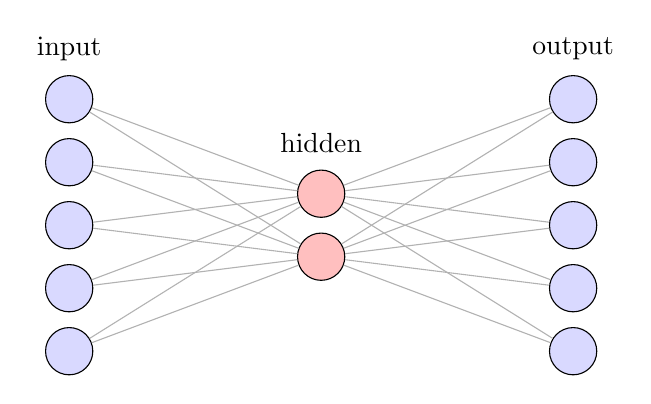
\begin{tikzpicture}[
    neuron/.style={circle,draw,minimum size=6mm,inner sep=0pt},
    edge/.style={gray!60},
    x=1.6cm,y=0.8cm]

  % input layer
  \foreach \i in {1,...,5}
    \node[neuron,fill=blue!15] (x\i) at (0,3-\i) {};

  % bottleneck
  \foreach \i in {1,2}
    \node[neuron,fill=red!25] (z\i) at (2,1.5-\i) {};

  % output layer
  \foreach \i in {1,...,5}
    \node[neuron,fill=blue!15] (y\i) at (4,3-\i) {};

  % connections
  \foreach \i in {1,...,5}
    \foreach \j in {1,2} {
      \draw[edge] (x\i) -- (z\j);
      \draw[edge] (z\j) -- (y\i);
    }

  % labels
  \node at (0,2.8)  {input};
  \node at (2,1.3)  {hidden};
  \node at (4,2.8)  {output};

\end{tikzpicture}
\end{center}
\end{frame}

\begin{frame}
  \frametitle{Motivation}
\vskip 0.25cm
\textbf{T}his is obviously nicely simple but it clearly fails to exploit the structure of day.
\end{frame}

\begin{frame}
  \frametitle{Vision}
\vskip 0.25cm
\textbf{T}he limitations of all-to-all networks was first obvious for vision, these days we forget but before GPT2 a lot of the focus in machine learning was on vision!
\end{frame}

\begin{frame}
  \frametitle{A challenge: CIFAR-10}
\vskip 0.25cm
\begin{center}
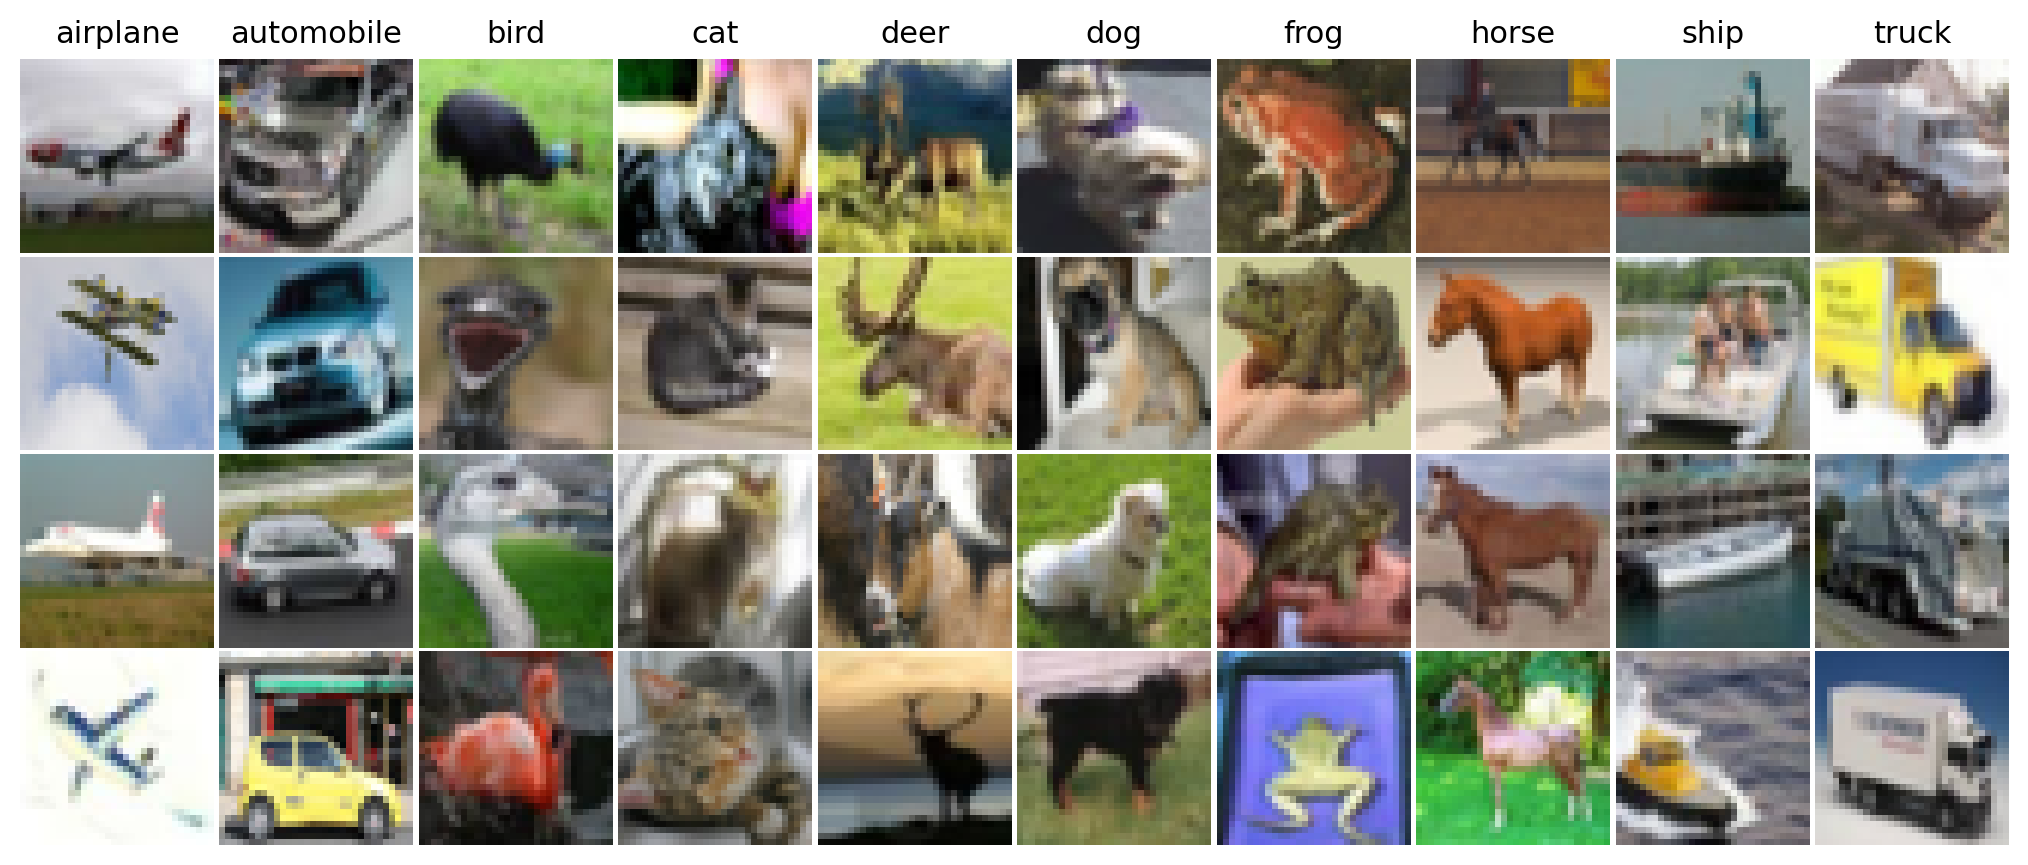
\includegraphics[width=0.9\textwidth]{cifar_grid.png}
\end{center}
\vskip 0.1cm
\textbf{S}ixty thousand tiny colour images, $32\times32$ pixels, in ten classes: airplane, automobile, bird, cat, deer, dog, frog, horse, ship, truck. That's 6,000 per class, split 50,000 for training and 10,000 for testing (Krizhevsky, 2009).
\vskip 0.2cm
\textbf{A}s a vector each image is just $32\times32\times3=3072$ numbers, and the cat can be anywhere in the frame, any size, facing any way, against any background.
\end{frame}

\begin{frame}
  \frametitle{The hierarchy idea}
\vskip 0.5cm
\begin{center}
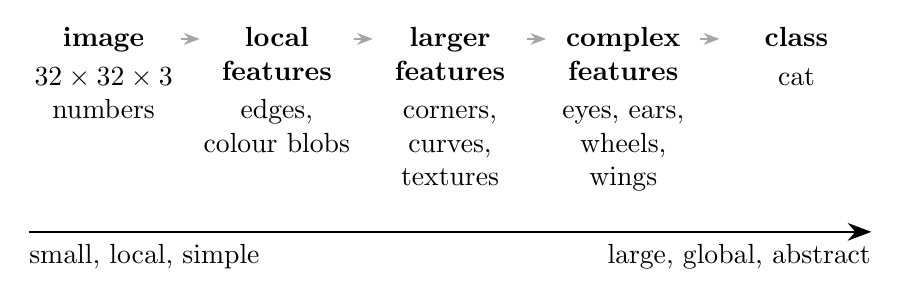
\begin{tikzpicture}[
    stage/.style={align=center,text width=1.9cm,inner sep=0pt,anchor=north},
    arr/.style={-{Stealth[length=2mm]},thick,gray!70}]

  % centres 2.2cm apart; arrows sit level with the first (bold) line
  \node[stage] (s0) at (0,0) {\textbf{image}\\[2pt] $32\times32\times3$ numbers};
  \onslide<2->{
  \node[stage] (s1) at (2.2,0) {\textbf{local features}\\[2pt] edges, colour blobs};
  \draw[arr] (0.98,-0.15) -- (1.22,-0.15);}
  \onslide<3->{
  \node[stage] (s2) at (4.4,0) {\textbf{larger features}\\[2pt] corners, curves, textures};
  \draw[arr] (3.18,-0.15) -- (3.42,-0.15);}
  \onslide<4->{
  \node[stage] (s3) at (6.6,0) {\textbf{complex features}\\[2pt] eyes, ears, wheels, wings};
  \draw[arr] (5.38,-0.15) -- (5.62,-0.15);}
  \onslide<5->{
  \node[stage] (s4) at (8.8,0) {\textbf{class}\\[2pt] cat};
  \draw[arr] (7.58,-0.15) -- (7.82,-0.15);}

  \onslide<6->{
  \draw[-{Stealth[length=3mm]},thick] (-0.95,-2.6) -- (9.75,-2.6);
  \node[anchor=north west,inner sep=0pt] at (-0.95,-2.75) {small, local, simple};
  \node[anchor=north east,inner sep=0pt] at (9.75,-2.75) {large, global, abstract};}
\end{tikzpicture}
\end{center}
\vskip 0.3cm
\onslide<6->{
\textbf{E}ach stage only looks at a small neighbourhood of the stage before, but because the stages stack, what each unit ``sees'' of the original image grows as we go up.
}
\end{frame}

\begin{frame}
  \frametitle{The brain got there first}
\vskip 0.1cm
\begin{center}
\begin{tikzpicture}[spike/.style={thick,blue!70}]

  % ---------------- screen with bar
  \draw[thick,fill=gray!10] (-0.9,-0.9) rectangle (0.9,0.9);
  \draw[thick] (0,-0.9) -- (0,-1.2);
  \draw[thick] (-0.4,-1.2) -- (0.4,-1.2);
  \only<1>{\fill[black,rotate around={0:(0,0)}]  (-0.55,-0.07) rectangle (0.55,0.07);}
  \only<2>{\fill[black,rotate around={45:(0,0)}] (-0.55,-0.07) rectangle (0.55,0.07);}
  \only<3->{\fill[black,rotate around={90:(0,0)}] (-0.55,-0.07) rectangle (0.55,0.07);}
  \node[below] at (0,-1.25) {stimulus};

  % ---------------- cat head in profile, facing left
  \begin{scope}[shift={(3.0,0)}]
    \fill[orange!25,draw=black,thick] (0,0) circle (0.8);
    \fill[orange!25,draw=black,thick] (-0.15,0.72) -- (0.0,1.3) -- (0.4,0.62) -- cycle;   % ear
    \fill[orange!25,draw=black,thick] (-0.62,-0.45) .. controls (-1.15,-0.35) and (-1.15,0.05) .. (-0.72,0.25)
          -- (-0.5,0) -- cycle;                                                            % snout
    \fill[black] (-1.03,-0.12) circle (0.06);                                            % nose
    \fill[black] (-0.35,0.25) ellipse (0.06 and 0.11);                                  % eye
    \draw[gray] (-0.85,-0.3) -- (-1.35,-0.2) (-0.85,-0.33) -- (-1.33,-0.42);            % whiskers
    \fill[orange!25] (-0.5,-0.42) -- (-0.5,0.02) -- (-0.68,0.22) -- (-0.6,-0.43) -- cycle; % hide seam
    % visual cortex, at the back of the head
    \fill[red!40,opacity=0.7] (0.55,-0.05) ellipse (0.18 and 0.3);
    % electrode
    \draw[very thick,gray!70!black] (0.55,0.0) -- (1.0,1.5);
    \fill[gray!70!black] (0.55,0.0) circle (0.04);
    \node[anchor=west,red!60!black] at (0.8,-0.55) {V1};
  \end{scope}

  % sight line
  \draw[dashed,gray] (0.9,0) -- (2.6,0.25);

  % ---------------- spike recording
  \begin{scope}[shift={(4.0,1.5)}]
    \draw[thick] (0,0) -- (2.2,0);
    \only<1>{\foreach \t in {0.6,1.7} \draw[spike] (\t,0) -- (\t,0.4);}
    \only<2>{\foreach \t in {0.25,0.7,1.1,1.55,1.95} \draw[spike] (\t,0) -- (\t,0.4);}
    \only<3->{\foreach \t in {0.1,0.22,0.35,0.48,0.6,0.72,0.85,0.98,1.1,1.22,1.35,1.48,1.6,1.72,1.85,1.98,2.1} \draw[spike] (\t,0) -- (\t,0.4);}
    \node[anchor=north] at (1.1,-0.05) {spikes};
  \end{scope}

  % ---------------- tuning curve
  \begin{scope}[shift={(7.0,-0.9)}]
    \draw[-{Stealth[length=2mm]}] (0,0) -- (3.0,0);
    \draw[-{Stealth[length=2mm]}] (0,0) -- (0,2.4);
    \node[anchor=south west] at (0.05,2.4) {firing rate};
    \foreach \x/\l in {0/0^\circ,1.4/90^\circ,2.8/180^\circ}
      \node[below] at (\x,0) {$\l$};
    \node at (1.4,-0.75) {bar angle};
    \onslide<4->{\draw[thick,red!70,domain=0:2.8,samples=60,smooth]
      plot (\x,{0.2+1.8*exp(-((\x-1.4)^2)/(2*0.53^2))});}
    \fill[blue!70] (0,0.25) circle (0.06);
    \onslide<2->{\fill[blue!70] (0.7,0.95) circle (0.06);}
    \onslide<3->{\fill[blue!70] (1.4,2.0) circle (0.06);}
  \end{scope}

\end{tikzpicture}
\end{center}
\vskip 0.1cm
\onslide<4->{
\textbf{H}ubel and Wiesel (1959) recorded single neurons in the visual cortex of anaesthetised cats: each cell fires for a bar at one orientation, in one small patch of the visual field.
}
\end{frame}

\begin{frame}
  \frametitle{The brain got there first}
\vskip 0.25cm
\textbf{S}imple cells respond to an oriented edge at one particular place, and the same detector is repeated across the whole visual field: this is a convolutional filter.
\vskip 0.2cm
\textbf{C}omplex cells respond to the same orientation anywhere within a larger patch, so they don't mind exactly where the edge is: this is pooling.
\vskip 0.2cm
\textbf{F}urther along the visual pathway cells respond to bigger and more complicated things, all the way up to faces in inferotemporal cortex: this is the hierarchy.
\vskip 0.2cm
\textbf{F}ukushima's neocognitron (1980) was built directly on this picture, and LeCun's convolutional networks followed from it.
\end{frame}

\begin{frame}
  \frametitle{Learning the same thing again and again}
\vskip 0.1cm
\begin{center}
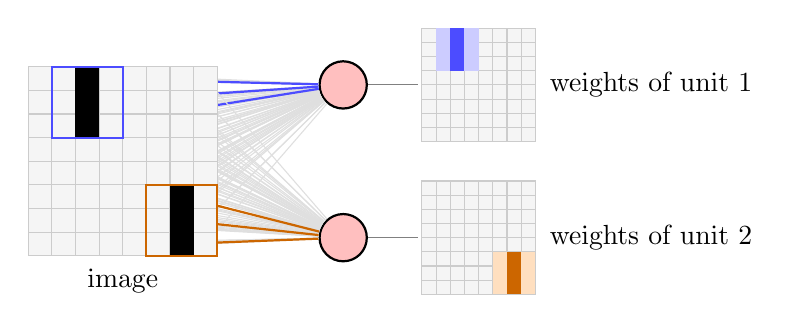
\begin{tikzpicture}[neuron/.style={circle,draw,thick,minimum size=6mm,inner sep=0pt,fill=red!25}]

  \node[neuron] (h1) at (4.0,1.97) {};
  \onslide<2->{\node[neuron] (h2) at (4.0,0.03) {};}

  % ---------------- connections (drawn first, so the image sits on top)
  \foreach \i in {0,...,7}
    \foreach \j in {0,...,7}
      \draw[gray!25] (0.3*\i+0.15,-0.05+0.3*\j) -- (h1);
  \foreach \j in {5,6,7} \draw[thick,blue!70] (0.75,-0.05+0.3*\j) -- (h1);
  \onslide<2->{
  \foreach \i in {0,...,7}
    \foreach \j in {0,...,7}
      \draw[gray!25] (0.3*\i+0.15,-0.05+0.3*\j) -- (h2);
  \foreach \j in {0,1,2} \draw[thick,orange!80!black] (1.95,-0.05+0.3*\j) -- (h2);}

  % ---------------- image: 8x8 pixels
  \foreach \i in {0,...,7}
    \foreach \j in {0,...,7}
      \draw[gray!40,fill=gray!8] (0.3*\i,-0.2+0.3*\j) rectangle ++(0.3,0.3);
  \foreach \j in {5,6,7} \fill[black] (0.6,-0.2+0.3*\j) rectangle ++(0.3,0.3);
  \draw[thick,blue!70] (0.3,1.3) rectangle (1.2,2.2);
  \onslide<2->{
  \foreach \j in {0,1,2} \fill[black] (1.8,-0.2+0.3*\j) rectangle ++(0.3,0.3);
  \draw[thick,orange!80!black] (1.5,-0.2) rectangle (2.4,0.7);}
  \node[below] at (1.2,-0.25) {image};

  % ---------------- weights of unit 1
  \begin{scope}[shift={(5.0,1.25)}]
    \foreach \i in {0,...,7}
      \foreach \j in {0,...,7}
        \draw[gray!40,fill=gray!8] (0.18*\i,0.18*\j) rectangle ++(0.18,0.18);
    \foreach \j in {5,6,7} {
      \fill[blue!20] (0.18,0.18*\j) rectangle ++(0.18,0.18);
      \fill[blue!70] (0.36,0.18*\j) rectangle ++(0.18,0.18);
      \fill[blue!20] (0.54,0.18*\j) rectangle ++(0.18,0.18);}
    \node[right] at (1.5,0.72) {weights of unit 1};
  \end{scope}
  \draw[gray] (h1) -- (4.95,1.97);

  % ---------------- weights of unit 2
  \onslide<2->{
  \begin{scope}[shift={(5.0,-0.69)}]
    \foreach \i in {0,...,7}
      \foreach \j in {0,...,7}
        \draw[gray!40,fill=gray!8] (0.18*\i,0.18*\j) rectangle ++(0.18,0.18);
    \foreach \j in {0,1,2} {
      \fill[orange!25] (0.9,0.18*\j) rectangle ++(0.18,0.18);
      \fill[orange!80!black] (1.08,0.18*\j) rectangle ++(0.18,0.18);
      \fill[orange!25] (1.26,0.18*\j) rectangle ++(0.18,0.18);}
    \node[right] at (1.5,0.72) {weights of unit 2};
  \end{scope}
  \draw[gray] (h2) -- (4.95,0.03);}

\end{tikzpicture}
\end{center}
\vskip 0.2cm
\onslide<1->{\textbf{U}nit 1 has learned to detect a vertical bar, but only in the top left: it has a separate weight for every pixel.}
\vskip 0.1cm
\onslide<2->{\textbf{T}o see the same bar in the bottom right, unit 2 has to learn it again from scratch, from examples where the bar happens to be there.}
\vskip 0.1cm
\onslide<3->{$\ldots$ and again for every other position, and for every other feature!}
\end{frame}

\begin{frame}
  \frametitle{Idea}
\vskip 0.1cm
\textbf{L}earn a single \emph{feature detector}, a small set of weights, and slide it across the whole image, so it responds to its feature wherever it appears.
\vskip 0.2cm
\begin{center}
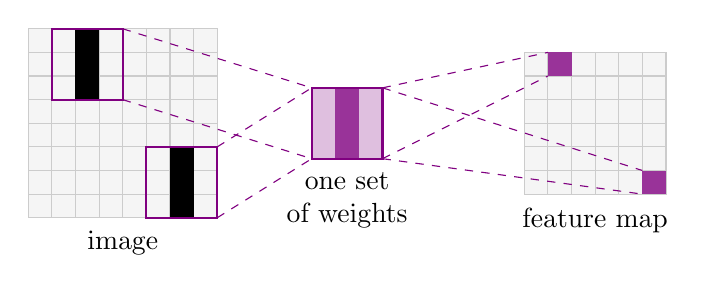
\begin{tikzpicture}
  % ---------------- image: 8x8
  \foreach \i in {0,...,7}
    \foreach \j in {0,...,7}
      \draw[gray!40,fill=gray!8] (0.3*\i,0.3*\j) rectangle ++(0.3,0.3);
  \foreach \j in {5,6,7} \fill[black] (0.6,0.3*\j) rectangle ++(0.3,0.3);
  \foreach \j in {0,1,2} \fill[black] (1.8,0.3*\j) rectangle ++(0.3,0.3);
  \node[below] at (1.2,-0.05) {image};

  % ---------------- the one filter
  \begin{scope}[shift={(3.6,0.75)}]
    \foreach \i in {0,1,2}
      \foreach \j in {0,1,2}
        \draw[gray!40,fill=gray!8] (0.3*\i,0.3*\j) rectangle ++(0.3,0.3);
    \foreach \j in {0,1,2} {
      \fill[violet!25] (0,0.3*\j) rectangle ++(0.3,0.3);
      \fill[violet!80] (0.3,0.3*\j) rectangle ++(0.3,0.3);
      \fill[violet!25] (0.6,0.3*\j) rectangle ++(0.3,0.3);}
    \draw[thick,violet] (0,0) rectangle (0.9,0.9);
    \node[below,align=center] at (0.45,-0.05) {one set\\of weights};
  \end{scope}

  % ---------------- feature map: 6x6
  \begin{scope}[shift={(6.3,0.3)}]
    \foreach \i in {0,...,5}
      \foreach \j in {0,...,5}
        \draw[gray!40,fill=gray!8] (0.3*\i,0.3*\j) rectangle ++(0.3,0.3);
    \onslide<2->{\fill[violet!80] (0.3,1.5) rectangle ++(0.3,0.3);}
    \onslide<3->{\fill[violet!80] (1.5,0) rectangle ++(0.3,0.3);}
    \node[below] at (0.9,-0.05) {feature map};
  \end{scope}

  % ---------------- top-left application
  \onslide<2->{
  \draw[thick,violet] (0.3,1.5) rectangle (1.2,2.4);
  \draw[violet,dashed] (1.2,2.4) -- (3.6,1.65);
  \draw[violet,dashed] (1.2,1.5) -- (3.6,0.75);
  \draw[violet,dashed] (4.5,1.65) -- (6.6,2.1);
  \draw[violet,dashed] (4.5,0.75) -- (6.6,1.8);}
  % ---------------- bottom-right application
  \onslide<3->{
  \draw[thick,violet] (1.5,0) rectangle (2.4,0.9);
  \draw[violet,dashed] (2.4,0.9) -- (3.6,1.65);
  \draw[violet,dashed] (2.4,0) -- (3.6,0.75);
  \draw[violet,dashed] (4.5,1.65) -- (7.8,0.6);
  \draw[violet,dashed] (4.5,0.75) -- (7.8,0.3);}
\end{tikzpicture}
\end{center}
\vskip 0.1cm
\onslide<4->{
\textbf{T}he same nine weights are used at every position: learn the bar once, detect it everywhere. This is a \emph{convolution}.
}
\end{frame}

\begin{frame}
  \frametitle{A simple convolutional network}
\vskip 0.3cm
\begin{center}
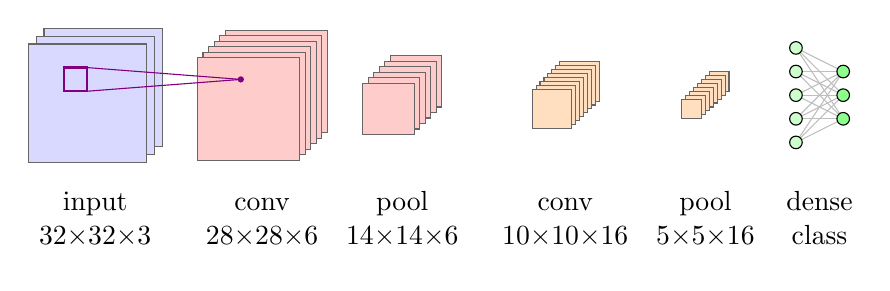
\begin{tikzpicture}[lab/.style={align=center,anchor=north,execute at begin node=\strut}]

  % input 32x32x3
  \foreach \k in {2,...,0}
    \draw[draw=black!60,fill=blue!15] (0+0.1*\k,-0.850+0.1*\k) rectangle ++(1.5,1.5);
  \node[lab] at (0.85,-1.05) {input\strut\\$32{\times}32{\times}3$};

  % conv 1: 28x28x6
  \onslide<2->{
  \foreach \k in {5,...,0}
    \draw[draw=black!60,fill=red!20] (2.15+0.07*\k,-0.825+0.07*\k) rectangle ++(1.3,1.3);
  \node[lab] at (2.97,-1.05) {conv\strut\\$28{\times}28{\times}6$};
  \draw[thick,violet] (0.45,0.05) rectangle ++(0.3,0.3);
  \draw[violet] (0.75,0.35) -- (2.7,0.2);
  \draw[violet] (0.75,0.05) -- (2.7,0.2);
  \fill[violet] (2.7,0.2) circle (0.04);}

  % pool 1: 14x14x6
  \onslide<3->{
  \foreach \k in {5,...,0}
    \draw[draw=black!60,fill=red!20] (4.25+0.07*\k,-0.500+0.07*\k) rectangle ++(0.65,0.65);
  \node[lab] at (4.75,-1.05) {pool\strut\\$14{\times}14{\times}6$};}

  % conv 2: 10x10x16 (drawn as 8 maps)
  \onslide<4->{
  \foreach \k in {7,...,0}
    \draw[draw=black!60,fill=orange!25] (6.4+0.05*\k,-0.425+0.05*\k) rectangle ++(0.5,0.5);
  \node[lab] at (6.82,-1.05) {conv\strut\\$10{\times}10{\times}16$};}

  % pool 2: 5x5x16
  \onslide<5->{
  \foreach \k in {7,...,0}
    \draw[draw=black!60,fill=orange!25] (8.3+0.05*\k,-0.300+0.05*\k) rectangle ++(0.25,0.25);
  \node[lab] at (8.6,-1.05) {pool\strut\\$5{\times}5{\times}16$};}

  % all-to-all layers and output
  \onslide<6->{
  \foreach \a in {-0.6,-0.3,...,0.7}
    \foreach \b in {-0.3,0,...,0.4}
      \draw[gray!50] (9.75,\a) -- (10.35,\b);
  \foreach \y in {-0.6,-0.3,...,0.7} \draw[fill=green!20] (9.75,\y) circle (0.08);
  \foreach \y in {-0.3,0,...,0.4} \draw[fill=green!45] (10.35,\y) circle (0.08);
  \node[lab] at (10.05,-1.05) {dense\strut\\class};}
\end{tikzpicture}
\end{center}
\vskip 0.2cm
\onslide<7->{
\textbf{C}onvolution finds features, pooling shrinks the maps so the next layer sees a larger patch of the image, and at the end an ordinary all-to-all layer picks the class. These are the sizes from LeCun's LeNet-5 (1998).
}
\end{frame}

\begin{frame}
  \frametitle{Convolution}
\vskip 0.1cm
\begin{center}
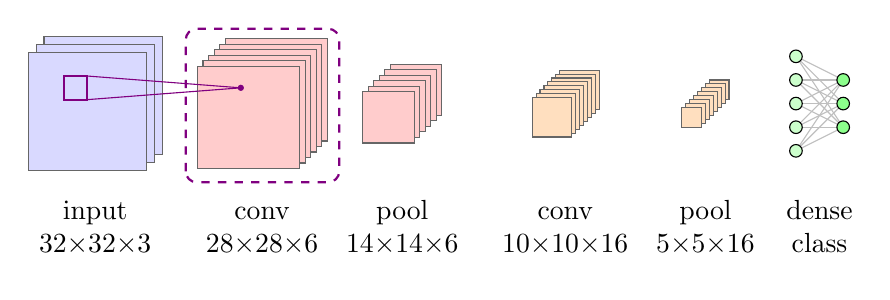
\begin{tikzpicture}[lab/.style={align=center,anchor=north,execute at begin node=\strut}]

  % input 32x32x3
  \foreach \k in {2,...,0}
    \draw[draw=black!60,fill=blue!15] (0+0.1*\k,-0.850+0.1*\k) rectangle ++(1.5,1.5);
  \node[lab] at (0.85,-1.05) {input\strut\\$32{\times}32{\times}3$};

  % conv 1: 28x28x6
  {
  \foreach \k in {5,...,0}
    \draw[draw=black!60,fill=red!20] (2.15+0.07*\k,-0.825+0.07*\k) rectangle ++(1.3,1.3);
  \node[lab] at (2.97,-1.05) {conv\strut\\$28{\times}28{\times}6$};
  \draw[thick,violet] (0.45,0.05) rectangle ++(0.3,0.3);
  \draw[violet] (0.75,0.35) -- (2.7,0.2);
  \draw[violet] (0.75,0.05) -- (2.7,0.2);
  \fill[violet] (2.7,0.2) circle (0.04);}

  % pool 1: 14x14x6
  {
  \foreach \k in {5,...,0}
    \draw[draw=black!60,fill=red!20] (4.25+0.07*\k,-0.500+0.07*\k) rectangle ++(0.65,0.65);
  \node[lab] at (4.75,-1.05) {pool\strut\\$14{\times}14{\times}6$};}

  % conv 2: 10x10x16 (drawn as 8 maps)
  {
  \foreach \k in {7,...,0}
    \draw[draw=black!60,fill=orange!25] (6.4+0.05*\k,-0.425+0.05*\k) rectangle ++(0.5,0.5);
  \node[lab] at (6.82,-1.05) {conv\strut\\$10{\times}10{\times}16$};}

  % pool 2: 5x5x16
  {
  \foreach \k in {7,...,0}
    \draw[draw=black!60,fill=orange!25] (8.3+0.05*\k,-0.300+0.05*\k) rectangle ++(0.25,0.25);
  \node[lab] at (8.6,-1.05) {pool\strut\\$5{\times}5{\times}16$};}

  % all-to-all layers and output
  {
  \foreach \a in {-0.6,-0.3,...,0.7}
    \foreach \b in {-0.3,0,...,0.4}
      \draw[gray!50] (9.75,\a) -- (10.35,\b);
  \foreach \y in {-0.6,-0.3,...,0.7} \draw[fill=green!20] (9.75,\y) circle (0.08);
  \foreach \y in {-0.3,0,...,0.4} \draw[fill=green!45] (10.35,\y) circle (0.08);
  \node[lab] at (10.05,-1.05) {dense\strut\\class};}
  % highlight
  \draw[thick,violet,dashed,rounded corners] (2.0,-1.0) rectangle (3.95,0.95);
\end{tikzpicture}
\end{center}
\textbf{C}onv:
\[
h^{c}_{ij}=\sigma\Big(\beta^{c}+\sum_{d=1}^{3}\,\sum_{k,l=0}^{4} w^{c}_{dkl}\;x^{d}_{i+k,\,j+l}\Big)
\]
\textbf{T}he weights $w^{c}_{dkl}$ don't depend on the position $i,j$: each of the six maps is one $5\times5\times3$ detector used everywhere, $456$ parameters in all, against about $14.5$ million for an all-to-all layer.
\end{frame}

\begin{frame}
  \frametitle{Pooling}
\vskip 0.1cm
\begin{center}
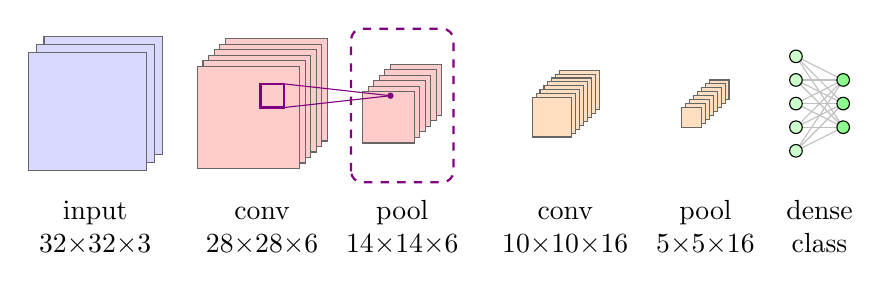
\begin{tikzpicture}[lab/.style={align=center,anchor=north,execute at begin node=\strut}]

  % input 32x32x3
  \foreach \k in {2,...,0}
    \draw[draw=black!60,fill=blue!15] (0+0.1*\k,-0.850+0.1*\k) rectangle ++(1.5,1.5);
  \node[lab] at (0.85,-1.05) {input\strut\\$32{\times}32{\times}3$};

  % conv 1: 28x28x6
  {
  \foreach \k in {5,...,0}
    \draw[draw=black!60,fill=red!20] (2.15+0.07*\k,-0.825+0.07*\k) rectangle ++(1.3,1.3);
  \node[lab] at (2.97,-1.05) {conv\strut\\$28{\times}28{\times}6$};
}

  % pool 1: 14x14x6
  {
  \foreach \k in {5,...,0}
    \draw[draw=black!60,fill=red!20] (4.25+0.07*\k,-0.500+0.07*\k) rectangle ++(0.65,0.65);
  \node[lab] at (4.75,-1.05) {pool\strut\\$14{\times}14{\times}6$};}

  % conv 2: 10x10x16 (drawn as 8 maps)
  {
  \foreach \k in {7,...,0}
    \draw[draw=black!60,fill=orange!25] (6.4+0.05*\k,-0.425+0.05*\k) rectangle ++(0.5,0.5);
  \node[lab] at (6.82,-1.05) {conv\strut\\$10{\times}10{\times}16$};}

  % pool 2: 5x5x16
  {
  \foreach \k in {7,...,0}
    \draw[draw=black!60,fill=orange!25] (8.3+0.05*\k,-0.300+0.05*\k) rectangle ++(0.25,0.25);
  \node[lab] at (8.6,-1.05) {pool\strut\\$5{\times}5{\times}16$};}

  % all-to-all layers and output
  {
  \foreach \a in {-0.6,-0.3,...,0.7}
    \foreach \b in {-0.3,0,...,0.4}
      \draw[gray!50] (9.75,\a) -- (10.35,\b);
  \foreach \y in {-0.6,-0.3,...,0.7} \draw[fill=green!20] (9.75,\y) circle (0.08);
  \foreach \y in {-0.3,0,...,0.4} \draw[fill=green!45] (10.35,\y) circle (0.08);
  \node[lab] at (10.05,-1.05) {dense\strut\\class};}
  % 2x2 block of the conv map pooled to one unit
  \draw[thick,violet] (2.95,-0.05) rectangle ++(0.3,0.3);
  \draw[violet] (3.25,0.25) -- (4.6,0.1);
  \draw[violet] (3.25,-0.05) -- (4.6,0.1);
  \fill[violet] (4.6,0.1) circle (0.04);
  % highlight
  \draw[thick,violet,dashed,rounded corners] (4.1,-1.0) rectangle (5.4,0.95);
\end{tikzpicture}
\end{center}
\textbf{P}ool:
\[
p^{c}_{ij}=\max_{k,l\in\{0,1\}}\, h^{c}_{2i+k,\,2j+l}
\]
\textbf{E}ach map is pooled separately over non-overlapping $2\times2$ blocks, with no weights to learn. The map halves in size, so the next convolution sees twice as far, and the output doesn't change if a feature moves by a pixel: like a complex cell.
\end{frame}

% preamble needs:
% \usepackage{tikz}
% \usepackage{listings}

\begin{frame}
  \frametitle{Example: MNIST}
\vskip 0.25cm
\begin{center}
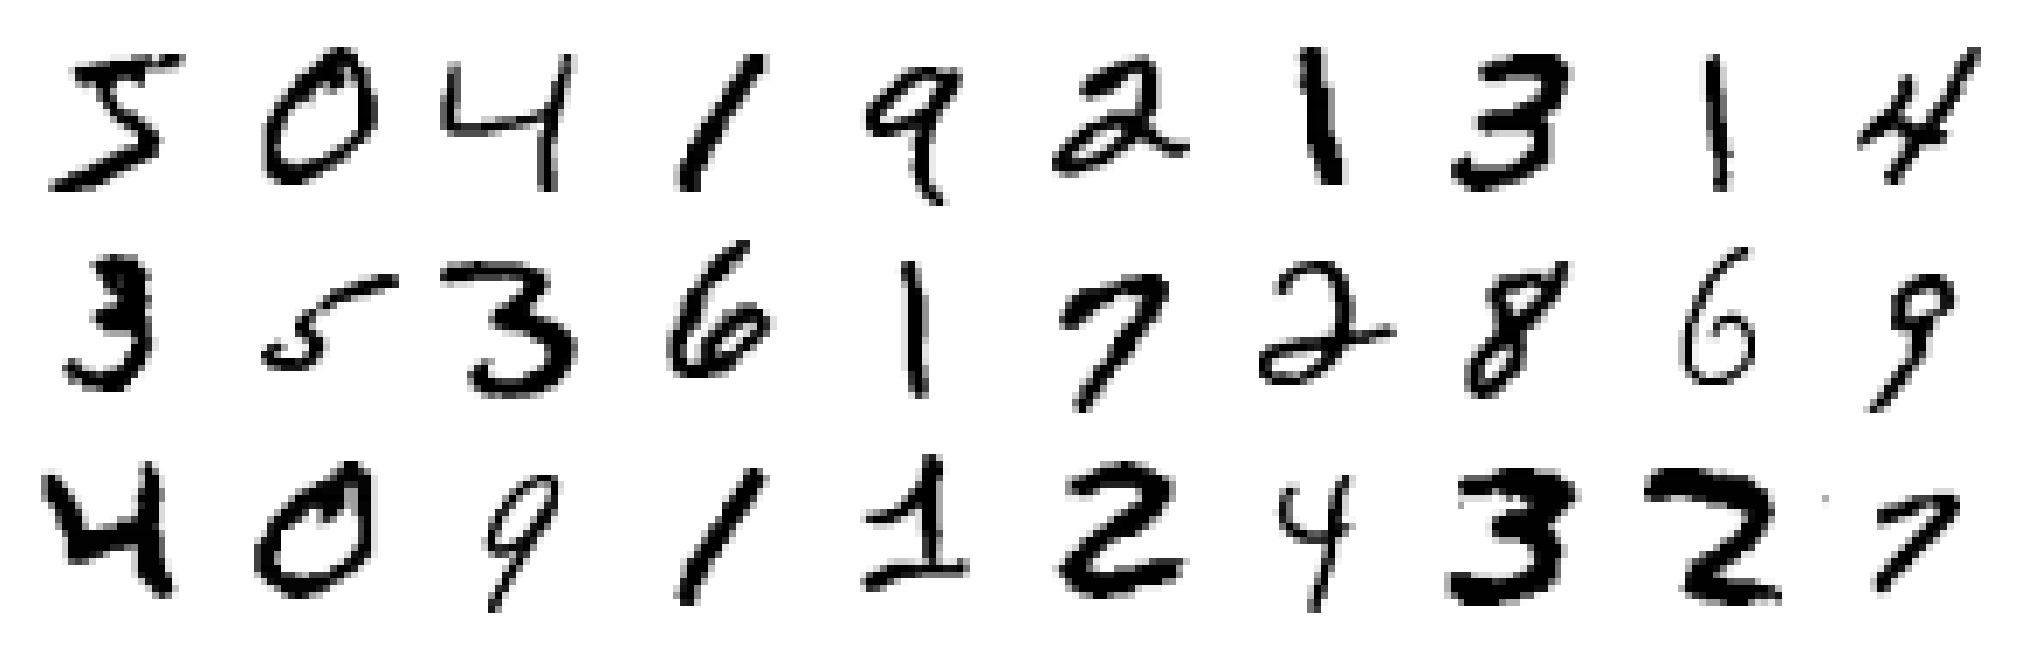
\includegraphics[width=0.85\textwidth]{mnist_grid.png}
\end{center}
\vskip 0.1cm
\textbf{H}andwritten digits, 0 to 9: 60,000 training images and 10,000 test images, each $28\times28$ pixels in greyscale (LeCun et al., 1998).
\vskip 0.2cm
\textbf{T}he ``hello world'' of image classification: small enough to train on a laptop in a minute or two.
\end{frame}

\begin{frame}
  \frametitle{A small CNN for MNIST}
\vskip 0.3cm
\begin{center}
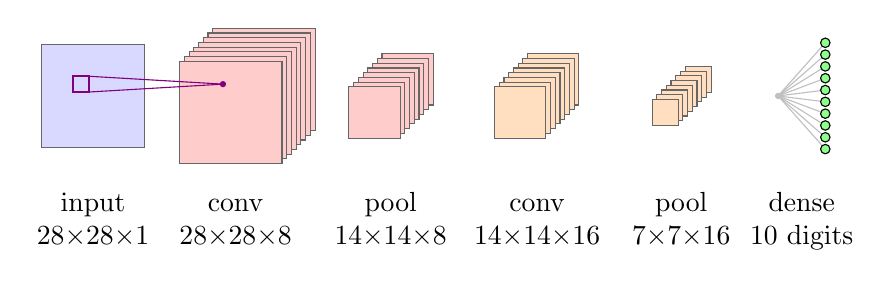
\begin{tikzpicture}[lab/.style={align=center,anchor=north,execute at begin node=\strut}]

  % input 28x28x1
  \draw[draw=black!60,fill=blue!15] (0,-0.65) rectangle ++(1.3,1.3);
  \node[lab] at (0.65,-1.05) {input\strut\\$28{\times}28{\times}1$};

  % conv 1: 28x28x8
  \foreach \k in {7,...,0}
    \draw[draw=black!60,fill=red!20] (1.75+0.06*\k,-0.86+0.06*\k) rectangle ++(1.3,1.3);
  \node[lab] at (2.46,-1.05) {conv\strut\\$28{\times}28{\times}8$};
  \draw[thick,violet] (0.4,0.05) rectangle ++(0.2,0.2);
  \draw[violet] (0.6,0.25) -- (2.3,0.15);
  \draw[violet] (0.6,0.05) -- (2.3,0.15);
  \fill[violet] (2.3,0.15) circle (0.04);

  % pool 1: 14x14x8
  \foreach \k in {7,...,0}
    \draw[draw=black!60,fill=red!20] (3.9+0.06*\k,-0.535+0.06*\k) rectangle ++(0.65,0.65);
  \node[lab] at (4.43,-1.05) {pool\strut\\$14{\times}14{\times}8$};

  % conv 2: 14x14x16 (drawn as 8 maps)
  \foreach \k in {7,...,0}
    \draw[draw=black!60,fill=orange!25] (5.75+0.06*\k,-0.535+0.06*\k) rectangle ++(0.65,0.65);
  \node[lab] at (6.29,-1.05) {conv\strut\\$14{\times}14{\times}16$};

  % pool 2: 7x7x16
  \foreach \k in {7,...,0}
    \draw[draw=black!60,fill=orange!25] (7.75+0.06*\k,-0.375+0.06*\k) rectangle ++(0.33,0.33);
  \node[lab] at (8.12,-1.05) {pool\strut\\$7{\times}7{\times}16$};

  % dense to 10 outputs
  \foreach \y in {-0.675,-0.525,...,0.7}
    \draw[gray!50] (9.35,0) -- (9.95,\y);
  \fill[gray!50] (9.35,0) circle (0.04);
  \foreach \y in {-0.675,-0.525,...,0.7} \draw[fill=green!45] (9.95,\y) circle (0.06);
  \node[lab] at (9.65,-1.05) {dense\strut\\10 digits};
\end{tikzpicture}
\end{center}
\vskip 0.2cm
\textbf{T}wo $3\times3$ convolutions, padded so they keep the size, each followed by a ReLU and a $2\times2$ max pool, then one all-to-all layer to the ten digits.
\vskip 0.2cm
\textbf{P}arameters: $80+1168+7850=9098$, most of them in the final dense layer.
\end{frame}

\begin{frame}
  \frametitle{Results}
\vskip 0.25cm
\textbf{A}fter three epochs, on the 10,000 test images:
\vskip 0.2cm
\begin{center}
\begin{tabular}{lcc}
 & parameters & test accuracy\\ \hline
small CNN & 9,098 & 98.0\% \\
all-to-all, one hidden layer of 12 & 9,550 & 93.2\% \\
\end{tabular}
\end{center}
\vskip 0.3cm
\textbf{T}he eight $3\times3$ filters the first layer learned:
\vskip 0.1cm
\begin{center}

\includegraphics[width=0.7\textwidth]{filters.png}
\end{center}
\end{frame}

\begin{frame}
  \frametitle{Text}
\vskip 0.3cm
\begin{center}
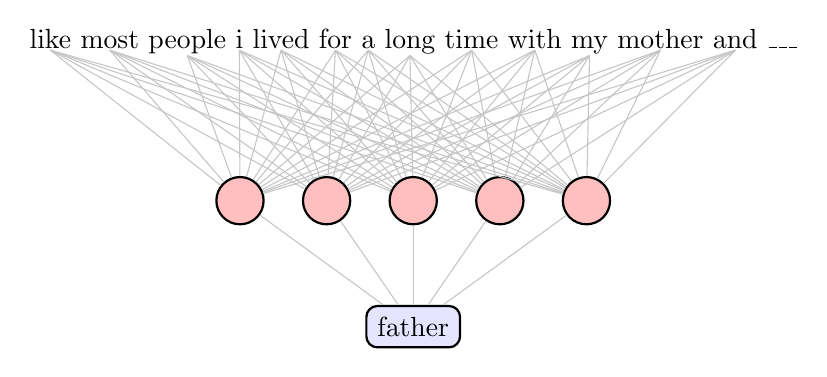
\begin{tikzpicture}[
    word/.style={inner sep=0.5pt,anchor=base west},
    neuron/.style={circle,draw,thick,minimum size=6mm,inner sep=0pt,fill=red!25},
    edge/.style={gray!45}]

  % the words, run along the top
  \node[word] (w1) at (0,0) {like};
  \foreach \w [count=\i from 2, remember=\i as \j (initially 1)] in
      {most,people,i,lived,for,a,long,time,with,my,mother,and}
    \node[word] (w\i) at ([xshift=0.07cm]w\j.base east) {\w};
  \node[word] (w14) at ([xshift=0.07cm]w13.base east) {\_\_\_};

  % hidden layer, centred under the sentence
  \path (w1.west) -- (w14.east) coordinate[midway] (mid);
  \foreach \h in {1,...,5}
    \node[neuron] (h\h) at ([xshift=(\h-3)*1.1cm,yshift=-2.0cm]mid) {};

  % all to all: every word to every hidden unit
  \foreach \i in {1,...,13}
    \foreach \h in {1,...,5}
      \draw[edge] (w\i.south) -- (h\h);

  % output
  \node[draw,thick,rounded corners,fill=blue!10,inner sep=4pt] (out) at ([yshift=-3.6cm]mid) {father};
  \foreach \h in {1,...,5}
    \draw[edge] (h\h) -- (out);
\end{tikzpicture}
\end{center}
\end{frame}

\begin{frame}
  \frametitle{Embeddings}
\vskip 0.1cm
\begin{center}
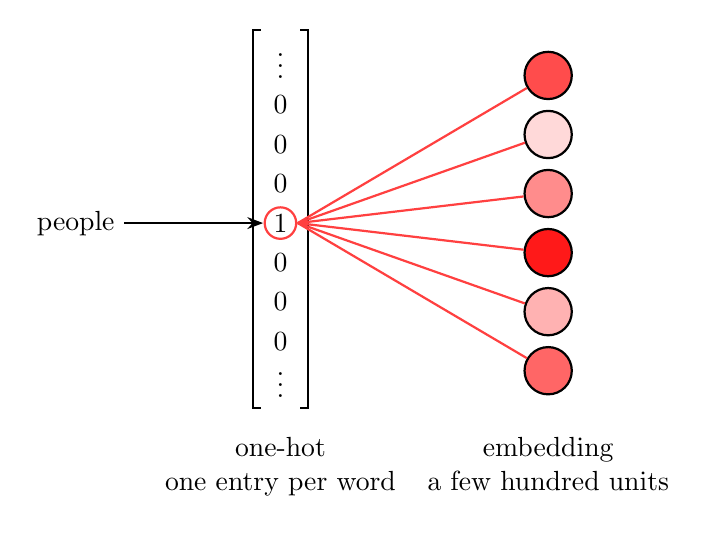
\begin{tikzpicture}[
    neuron/.style={circle,draw,thick,minimum size=6mm,inner sep=0pt}]

  % the word
  \node (word) at (0,0) {people};

  % one-hot column
  \foreach \y in {1.5,1.0,0.5,-0.5,-1.0,-1.5}
    \node at (2.6,\y) {$0$};
  \node (one) at (2.6,0) {$1$};
  \node at (2.6,2.1) {$\vdots$};
  \node at (2.6,-1.95) {$\vdots$};
  \draw[thick] (2.35,2.45) -- (2.25,2.45) -- (2.25,-2.35) -- (2.35,-2.35);
  \draw[thick] (2.85,2.45) -- (2.95,2.45) -- (2.95,-2.35) -- (2.85,-2.35);
  \draw[thick,red!75] (one) circle (0.2);

  % word points to its entry
  \draw[-{Stealth[length=2mm]},thick] (word) -- (2.38,0);

  % embedding layer
  \foreach \y/\s [count=\n] in {1.875/70,1.125/15,0.375/45,-0.375/90,-1.125/30,-1.875/60}
    \node[neuron,fill=red!\s] (e\n) at (6.0,\y) {};
  \foreach \n in {1,...,6}
    \draw[thick,red!75] (2.82,0) -- (e\n);

  % labels
  \node[align=center,anchor=north] at (2.6,-2.6) {one-hot\\one entry per word};
  \node[align=center,anchor=north] at (6.0,-2.6) {embedding\\a few hundred units};
\end{tikzpicture}
\end{center}
\end{frame}

\begin{frame}
  \frametitle{Text - the all-to-all problem again!}
\vskip 0.3cm
\begin{center}
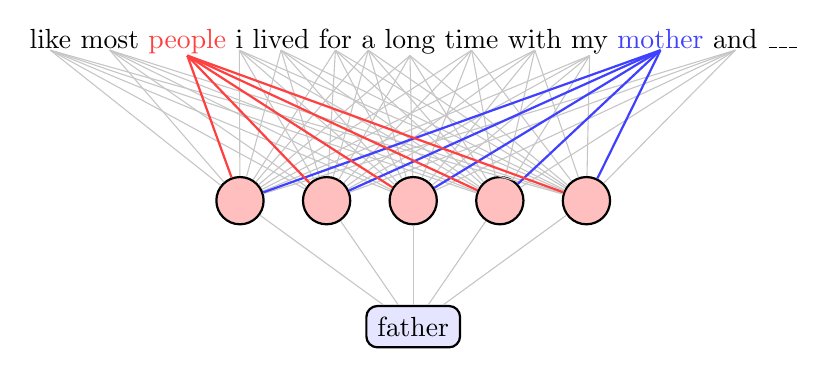
\begin{tikzpicture}[
    word/.style={inner sep=0.5pt,anchor=base west},
    neuron/.style={circle,draw,thick,minimum size=6mm,inner sep=0pt,fill=red!25},
    edge/.style={gray!45}]

  % the words, run along the top
  \node[word] (w1) at (0,0) {like};
  \foreach \w [count=\i from 2, remember=\i as \j (initially 1)] in
      {most,\textcolor{red!75}{people},i,lived,for,a,long,time,with,my,\textcolor{blue!75}{mother},and}
    \node[word] (w\i) at ([xshift=0.07cm]w\j.base east) {\w};
  \node[word] (w14) at ([xshift=0.07cm]w13.base east) {\_\_\_};

  % hidden layer, centred under the sentence
  \path (w1.west) -- (w14.east) coordinate[midway] (mid);
  \foreach \h in {1,...,5}
    \node[neuron] (h\h) at ([xshift=(\h-3)*1.1cm,yshift=-2.0cm]mid) {};

  % all to all: every word to every hidden unit
  \foreach \i in {1,2,4,5,6,7,8,9,10,11,13}
    \foreach \h in {1,...,5}
      \draw[edge] (w\i.south) -- (h\h);
  % weights from "people" in red, from "mother" in blue
  \foreach \h in {1,...,5} {
    \draw[thick,red!75] (w3.south) -- (h\h);
    \draw[thick,blue!75] (w12.south) -- (h\h);}

  % output
  \node[draw,thick,rounded corners,fill=blue!10,inner sep=4pt] (out) at ([yshift=-3.6cm]mid) {father};
  \foreach \h in {1,...,5}
    \draw[edge] (h\h) -- (out);
\end{tikzpicture}
\end{center}
\end{frame}

\begin{frame}
  \frametitle{Idea: RNN}
\vskip 0.3cm
\begin{center}
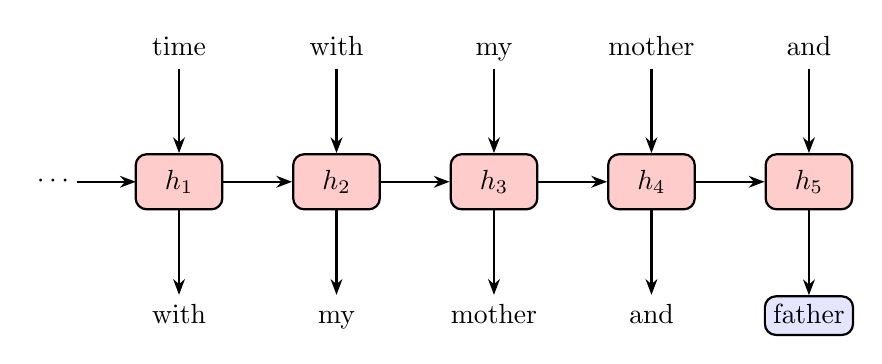
\begin{tikzpicture}[
    hid/.style={draw,thick,rounded corners,fill=red!20,minimum width=1.1cm,minimum height=0.7cm},
    arr/.style={-{Stealth[length=2mm]},thick},
    word/.style={text height=1.6ex,text depth=0.25ex}]

  % what came before
  \node at (-1.6,0) {$\cdots$};
  \draw[arr] (-1.3,0) -- (-0.55,0);

  \onslide<1->{
    \node[word] (x1) at (0.0,1.7) {time};
    \node[hid] (h1) at (0.0,0) {$h_1$};
    \node[word] (y1) at (0.0,-1.7) {with};
    \draw[arr] (x1) -- (h1);
    \draw[arr] (h1) -- (y1);}
  \onslide<2->{
    \node[word] (x2) at (2.0,1.7) {with};
    \node[hid] (h2) at (2.0,0) {$h_2$};
    \node[word] (y2) at (2.0,-1.7) {my};
    \draw[arr] (x2) -- (h2);
    \draw[arr] (h2) -- (y2);
    \draw[arr] (h1) -- (h2);}
  \onslide<3->{
    \node[word] (x3) at (4.0,1.7) {my};
    \node[hid] (h3) at (4.0,0) {$h_3$};
    \node[word] (y3) at (4.0,-1.7) {mother};
    \draw[arr] (x3) -- (h3);
    \draw[arr] (h3) -- (y3);
    \draw[arr] (h2) -- (h3);}
  \onslide<4->{
    \node[word] (x4) at (6.0,1.7) {mother};
    \node[hid] (h4) at (6.0,0) {$h_4$};
    \node[word] (y4) at (6.0,-1.7) {and};
    \draw[arr] (x4) -- (h4);
    \draw[arr] (h4) -- (y4);
    \draw[arr] (h3) -- (h4);}
  \onslide<5->{
    \node[word] (x5) at (8.0,1.7) {and};
    \node[hid] (h5) at (8.0,0) {$h_5$};
    \node[word,draw,rounded corners,fill=blue!10,inner sep=3pt,line width=0.8pt] (y5) at (8.0,-1.7) {father};
    \draw[arr] (x5) -- (h5);
    \draw[arr] (h5) -- (y5);
    \draw[arr] (h4) -- (h5);}
\end{tikzpicture}
\end{center}
\vskip 0.3cm
\onslide<6->{
\textbf{R}ead one word at a time: the hidden state $h_t$ carries forward what has been read so far, and the \emph{same} weights are used at every step.
}
\end{frame}

\begin{frame}
  \frametitle{Problems}
\vskip 0.25cm
\textbf{V}anishing gradients: the gradient reaching a word $k$ steps back is a product of $k$ factors,
\[
\frac{\partial h_t}{\partial h_{t-k}}=\prod_{s=t-k+1}^{t}\mathrm{diag}\big(\sigma'_s\big)\,W,
\]
and if these are mostly smaller than one it shrinks exponentially, so the network can't learn that something far back matters.
\vskip 0.2cm
\textbf{E}xploding gradients: if the factors are mostly bigger than one the same product blows up and training goes unstable; the usual patch is to clip the gradient.
\vskip 0.2cm
\end{frame}

\begin{frame}
  \frametitle{Problems}
\vskip 0.25cm
\textbf{O}ne fixed-size bottleneck: everything read so far has to be squeezed into the single vector $h_t$, and new words keep overwriting old ones.
\vskip 0.2cm
\textbf{S}trictly sequential: $h_t$ can't be computed until $h_{t-1}$ is done, so training can't be parallelised along the text and is slow on modern hardware.
\end{frame}

\begin{frame}
  \frametitle{LSTM}
\begin{center}
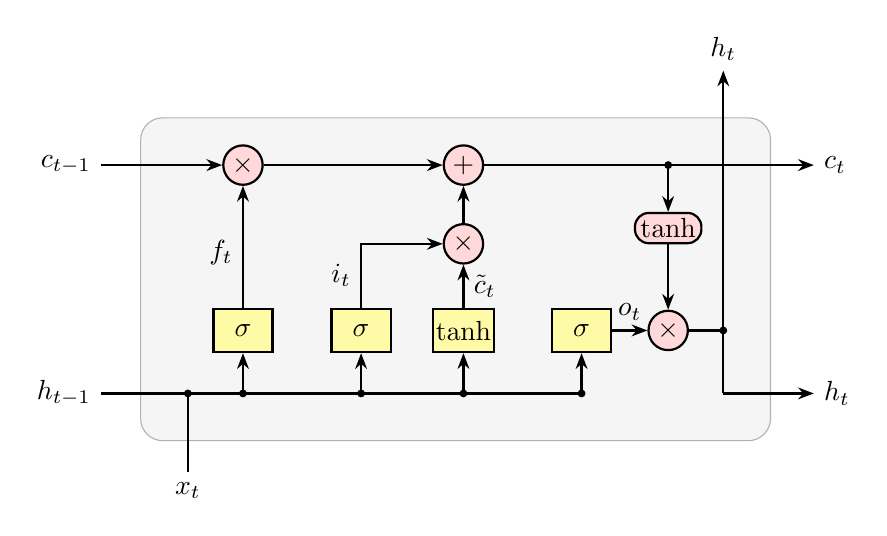
\begin{tikzpicture}[
    gate/.style={draw,thick,fill=yellow!35,minimum width=0.75cm,minimum height=0.55cm,inner sep=1pt},
    op/.style={circle,draw,thick,fill=red!15,minimum size=5mm,inner sep=0pt},
    tnh/.style={draw,thick,rounded corners=5pt,fill=red!15,inner sep=2pt},
    arr/.style={-{Stealth[length=2mm]},thick},
    line/.style={thick}]

  % the cell
  \draw[rounded corners=8pt,fill=gray!8,draw=gray!60] (0.2,-0.1) rectangle (8.2,4.0);

  % cell state, along the top
  \node[op] (fx) at (1.5,3.4) {$\times$};
  \node[op] (pl) at (4.3,3.4) {$+$};
  \draw[arr] (-0.3,3.4) node[left] {$c_{t-1}$} -- (fx);
  \draw[arr] (fx) -- (pl);
  \draw[arr] (pl) -- (8.75,3.4) node[right] {$c_t$};

  % hidden state and input, merged into one bus along the bottom
  \draw[line] (-0.3,0.5) node[left] {$h_{t-1}$} -- (5.8,0.5);
  \draw[line] (0.8,-0.5) node[below] {$x_t$} -- (0.8,0.5);
  \fill (0.8,0.5) circle (0.05);

  % the four layers
  \node[gate] (f) at (1.5,1.3) {$\sigma$};
  \node[gate] (i) at (3.0,1.3) {$\sigma$};
  \node[gate] (g) at (4.3,1.3) {$\tanh$};
  \node[gate] (o) at (5.8,1.3) {$\sigma$};
  \foreach \n/\x in {f/1.5,i/3.0,g/4.3,o/5.8} {
    \draw[arr] (\x,0.5) -- (\n);
    \fill (\x,0.5) circle (0.05);}

  % forget
  \draw[arr] (f) -- (fx) node[pos=0.45,left] {$f_t$};

  % input
  \node[op] (ix) at (4.3,2.4) {$\times$};
  \draw[arr] (i) |- (ix) node[pos=0.25,left] {$i_t$};
  \draw[arr] (g) -- (ix) node[midway,right] {$\tilde c_t$};
  \draw[arr] (ix) -- (pl);

  % output
  \node[tnh] (tc) at (6.9,2.6) {$\tanh$};
  \node[op] (ox) at (6.9,1.3) {$\times$};
  \draw[arr] (6.9,3.4) -- (tc);
  \fill (6.9,3.4) circle (0.05);
  \draw[arr] (tc) -- (ox);
  \draw[arr] (o) -- (ox) node[midway,above] {$o_t$};
  \draw[line] (ox) -| (7.6,0.5);
  \draw[arr] (7.6,0.5) -- (8.75,0.5) node[right] {$h_t$};
  \draw[arr] (7.6,1.3) -- (7.6,4.6) node[above] {$h_t$};
  \fill (7.6,1.3) circle (0.05);
\end{tikzpicture}
\end{center}
\textbf{T}he cell state $c_t$ runs along the top with only a $\times$ and a $+$ on it, so gradients can flow back many steps without being squashed.
\end{frame}

\begin{frame}
  \frametitle{Transformers}
\vskip 0.25cm
\textbf{H}owever, a different solution was found, almost by accident, one that solves the bottleneck and training problems too: the \emph{transformer}.
\end{frame}

\begin{frame}
  \frametitle{The task is the same}
\vskip 0.2cm
\begin{center}
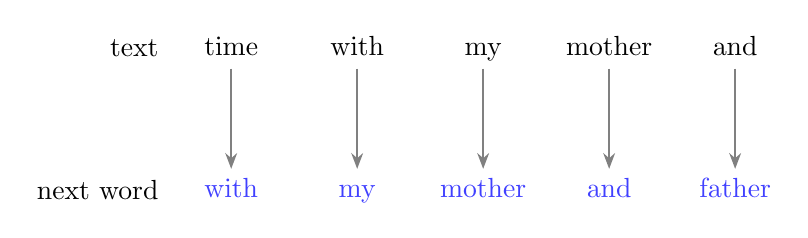
\begin{tikzpicture}[
    arr/.style={-{Stealth[length=2mm]},thick},
    word/.style={text height=1.6ex,text depth=0.25ex}]
  \node[anchor=east] at (-0.8,1.2) {text};
  \node[anchor=east] at (-0.8,-0.6) {next word};
  \foreach \w/\o [count=\t] in {time/with,with/my,my/mother,mother/and,and/father} {
    \pgfmathsetmacro\x{1.6*(\t-1)}
    \node[word] (x\t) at (\x,1.2) {\w};
    \node[word,text=blue!75] (y\t) at (\x,-0.6) {\o};
    \draw[arr,gray] (x\t) -- (y\t);
  }
\end{tikzpicture}
\end{center}
\vskip 0.2cm
\textbf{A}t every position, predict the next word, using only that word and the ones before it.
\vskip 0.2cm
\textbf{T}he next words are just the text shifted along by one, so any text is training data, and all the positions are trained \emph{at the same time}.
\vskip 0.2cm
\textbf{A} transformer does this in three steps: \emph{embed} each word, let the words \emph{attend} to each other, then \emph{predict}.
\end{frame}

\begin{frame}
  \frametitle{Step 1: embed}
\vskip 0.2cm
\begin{center}
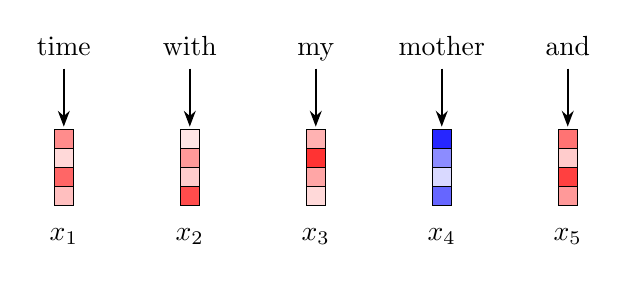
\begin{tikzpicture}[
    arr/.style={-{Stealth[length=2mm]},thick},
    word/.style={text height=1.6ex,text depth=0.25ex}]
  \foreach \w/\c/\sa/\sb/\sc/\sd [count=\t] in
      {time/red/25/60/15/45, with/red/70/20/40/10, my/red/15/35/80/30,
       mother/blue/60/15/45/85, and/red/40/75/20/55} {
    \pgfmathsetmacro\x{1.6*(\t-1)}
    \node[word] (x\t) at (\x,2.0) {\w};
    \foreach \k/\s in {0/\sa,1/\sb,2/\sc,3/\sd}
      \draw[fill=\c!\s] (\x-0.12,0+0.24*\k) rectangle ++(0.24,0.24);
    \draw[arr] (x\t) -- (\x,1.0);
    \node at (\x,-0.4) {$x_{\t}$};
  }
\end{tikzpicture}
\end{center}
\vskip 0.2cm
\textbf{E}very word is turned into a vector with the same embedding as before, so ``mother'' always starts from the same point, wherever it appears.
\vskip 0.2cm
\textbf{A} vector saying \emph{where} the word is, position 1, 2, 3, \dots, is added on, since otherwise nothing would record the order.
\end{frame}

\begin{frame}
  \frametitle{Step 2: attention, the idea}
\begin{center}
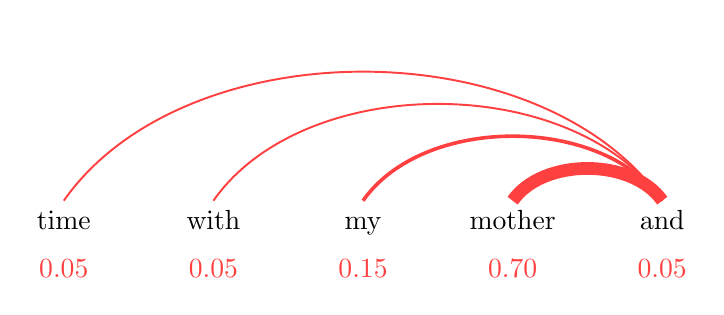
\begin{tikzpicture}[word/.style={text height=1.6ex,text depth=0.25ex}]
  \foreach \w [count=\t] in {time,with,my,mother,and}
    \node[word] (w\t) at (1.9*\t-1.9,0) {\w};
  \foreach \t/\a in {1/0.05,2/0.05,3/0.15,4/0.70}
    \draw[red!75,line width=\a*6pt+0.4pt] (w5.north) to[out=125,in=55,looseness=0.9] (w\t.north);
  % the weights, written under the words
  \foreach \t/\a in {1/0.05,2/0.05,3/0.15,4/0.70,5/0.05}
    \node[text=red!75] at (1.9*\t-1.9,-0.6) {\a};
\end{tikzpicture}
\end{center}
\textbf{T}o update the vector for ``and'', take a weighted average of vectors $v$, one from each word up to and including it:
\[
z_{\text{and}} = 0.05\,v_{\text{time}}+0.05\,v_{\text{with}}+0.15\,v_{\text{my}}+0.70\,v_{\text{mother}}+0.05\,v_{\text{and}}
\]
\textbf{T}he weights add up to one and say how relevant each word is here: to guess what comes after ``and'', ``mother'' matters most.
\end{frame}

\begin{frame}
  \frametitle{Step 2: attention, choosing the weights}
\vskip 0.2cm
\textbf{E}ach word $j$ makes three vectors from its own vector $x_j$, each by a learned linear map:
\vskip 0.1cm
\begin{center}
\begin{tabular}{rl}
query $q_j$: & what am I looking for?\\
key $k_j$: & what do I have to offer?\\
value $v_j$: & what do I pass on if chosen?
\end{tabular}
\end{center}
\vskip 0.1cm
\textbf{W}ord $i$ scores each word up to itself by how well its query matches that word's key, turns the scores into weights with a softmax, and averages the values:
\[
a_{ij}=\frac{e^{\,q_i\cdot k_j}}{\sum_{l\le i}e^{\,q_i\cdot k_l}},\qquad
z_i=\sum_{j\le i}a_{ij}\,v_j .
\]
\textbf{O}nly $j\le i$: a word may not look ahead at the word it is meant to predict.
\end{frame}

\begin{frame}
  \frametitle{Step 2: attention, queries and keys}
\begin{center}
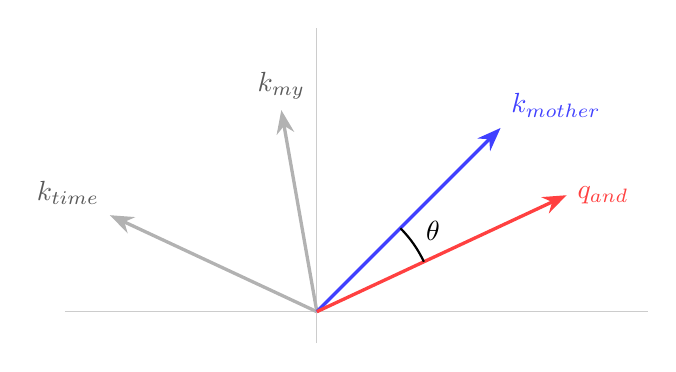
\begin{tikzpicture}[
    vecq/.style={-{Stealth[length=3mm]},very thick,red!75},
    veck/.style={-{Stealth[length=3mm]},very thick,blue!75},
    veco/.style={-{Stealth[length=3mm]},very thick,gray!60}]
  % faint axes
  \draw[gray!40] (-3.2,0) -- (4.2,0);
  \draw[gray!40] (0,-0.4) -- (0,3.6);

  % keys
  \draw[veco] (0,0) -- (155:2.9) node[above left,text=gray!70!black] {$k_{\text{time}}$};
  \draw[veco] (0,0) -- (100:2.6) node[above,text=gray!70!black] {$k_{\text{my}}$};
  \draw[veck] (0,0) -- (45:3.3) node[above right] {$k_{\text{mother}}$};
  % query
  \draw[vecq] (0,0) -- (25:3.5) node[right] {$q_{\text{and}}$};

  % the angle between query and the key for "mother"
  \draw[thick] (25:1.5) arc (25:45:1.5);
  \node at (35:1.8) {$\theta$};
\end{tikzpicture}
\end{center}
\textbf{T}he score is a dot product,
\[
q_i\cdot k_j=|q_i|\,|k_j|\cos\theta ,
\]
so it is large when the key points the same way as the query: a small angle means a big score and, after the softmax, a big weight.
\end{frame}

\begin{frame}
  \frametitle{Step 2: one block, attention then a network}
\begin{center}
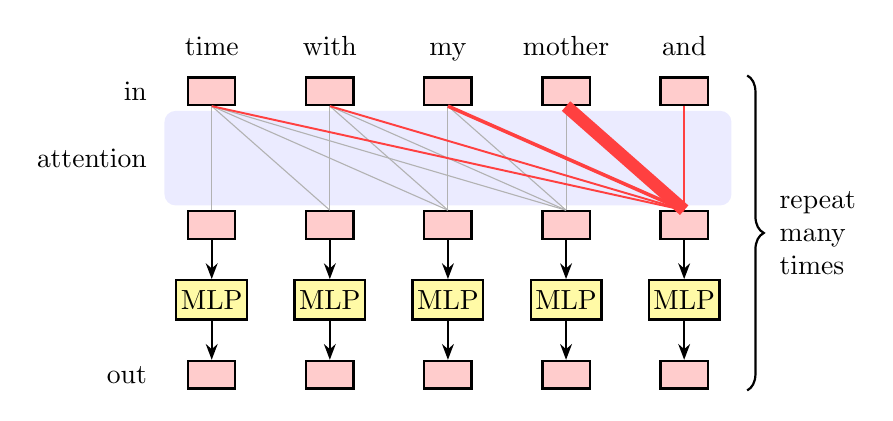
\begin{tikzpicture}[
    vec/.style={draw,thick,fill=red!20,minimum width=0.6cm,minimum height=0.35cm,inner sep=0pt},
    mlp/.style={draw,thick,fill=yellow!35,minimum width=0.9cm,minimum height=0.5cm,inner sep=1pt},
    arr/.style={-{Stealth[length=2mm]},thick},
    word/.style={text height=1.6ex,text depth=0.25ex}]

  % the attention band
  \fill[blue!8,rounded corners] (0.9,2.5) rectangle (8.1,3.7);

  \foreach \w [count=\t] in {time,with,my,mother,and} {
    \pgfmathsetmacro\x{1.5*\t}
    \node[word] at (\x,4.5) {\w};
    \node[vec] (a\t) at (\x,3.95) {};
    \node[vec] (b\t) at (\x,2.25) {};
    \node[mlp] (m\t) at (\x,1.3) {MLP};
    \node[vec] (c\t) at (\x,0.35) {};
    \draw[arr] (b\t) -- (m\t);
    \draw[arr] (m\t) -- (c\t);
  }
  % attention: each position reads from itself and every earlier position
  \foreach \i in {1,...,4}
    \foreach \j in {1,...,\i}
      \draw[gray!60] (a\j.south) -- (b\i.north);
  % the weights into "and", as on the earlier slide
  \foreach \j/\a in {1/0.05,2/0.05,3/0.15,4/0.70,5/0.05}
    \draw[red!75,line width=\a*6pt+0.4pt] (a\j.south) -- (b5.north);

  \node[anchor=east] at (0.8,3.95) {in};
  \node[anchor=east] at (0.8,3.1) {attention};
  \node[anchor=east] at (0.8,0.35) {out};
  \draw[decorate,decoration={brace,amplitude=6pt},thick] (8.3,4.15) -- (8.3,0.15)
    node[midway,right=8pt,align=left] {repeat\\many\\times};
\end{tikzpicture}
\end{center}
\textbf{A}ttention is the only place where information moves \emph{between} words; the red lines are the weights into ``and'' from before.
\vskip 0.1cm
\textbf{T}hen a small all-to-all network, an MLP, works on each word \emph{separately}, with the same weights at every position, like a convolution.
\end{frame}

\begin{frame}
  \frametitle{Step 3: predict}
\vskip 0.1cm
\begin{center}
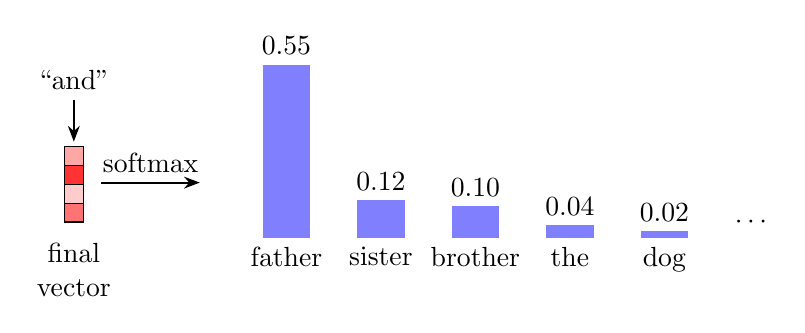
\begin{tikzpicture}[arr/.style={-{Stealth[length=2mm]},thick}]
  \node (and) at (0,1.2) {``and''};
  \foreach \k/\s in {0/55,1/20,2/80,3/35}
    \draw[fill=red!\s] (-0.12,-0.6+0.24*\k) rectangle ++(0.24,0.24);
  \draw[arr] (and) -- (0,0.42);
  \node[align=center,anchor=north] at (0,-0.75) {final\\vector};
  \draw[arr] (0.35,-0.1) -- (1.6,-0.1) node[midway,above] {softmax};
  % probabilities over the vocabulary
  \foreach \w/\p [count=\n] in {father/0.55,sister/0.12,brother/0.10,the/0.04,dog/0.02} {
    \pgfmathsetmacro\x{1.5+1.2*\n}
    \fill[blue!50] (\x-0.3,-0.8) rectangle ++(0.6,4*\p);
    \node[anchor=south] at (\x,-0.8+4*\p) {\p};
    \node[anchor=north] at (\x,-0.8) {\w};
  }
  \node at (8.6,-0.6) {$\cdots$};
\end{tikzpicture}
\end{center}
\vskip 0.1cm
\textbf{A}fter the last block, each position's vector goes through one more all-to-all layer with a softmax, giving a probability for every word in the vocabulary.
\vskip 0.1cm
\textbf{T}raining pushes up the probability of the word that actually came next: here, ``father''.
\end{frame}

\begin{frame}
  \frametitle{What the transformer gives us}
\vskip 0.25cm
\textbf{T}ransferable representations: the same embedding and the same weights at every position, so what is learned about a word in one place is used everywhere.
\vskip 0.2cm
\textbf{C}ontext: through attention, each word's vector is rebuilt from the words around it, so ``bank'' near ``river'' and ``bank'' near ``money'' end up different.
\vskip 0.2cm
\textbf{N}o bottleneck: any word can look straight back at any earlier word, rather than hoping it survived in $h_t$.
\vskip 0.2cm
\textbf{F}ast training: every position is computed at once with big matrix multiplications, which is exactly what GPUs are good at.
\end{frame}

\begin{frame}
  \frametitle{Now}
\vskip 0.25cm
\textbf{T}ransformers are now the only game in town!
\vskip 0.2cm
\textbf{L}anguage, obviously: every large language model is a transformer.
\vskip 0.2cm
\textbf{B}ut also vision, where an image is cut into patches and the patches are treated like words, and speech, protein structure, weather forecasting, robotics \dots
\vskip 0.2cm
\textbf{C}NNs and RNNs built in the structure of the data by hand; the transformer assumes much less and, given enough data, learns the structure for itself.
\end{frame}

\end{document}
